\subsection{Ragno Network}

The Ragno Network serves as the foundational layer of the Omnichain Web and emerged from a personal challenge we encountered with the initial V1 of the Dojima architecture. This is a challenge common to all cross-chain protocols, where adding a new chain requires each validator to either run a new node or update their RPC URLs—both costly and complex tasks. The Ragno Network is a cutting-edge protocol designed for interoperability between Layer 1 (L1) blockchains. It addresses key issues that hinder seamless interaction and communication across different blockchain ecosystems. By addressing fragmentation and inefficiencies in cross-chain operations, Ragno plays a crucial role in enabling interconnectedness, scalability, and security within decentralized networks. Its innovative architecture is central to the ongoing evolution of blockchain technology.

Ragno eliminates the need for centralized intermediaries by utilizing a decentralized protocol driven by a network of validators and relayers. This ensures that all cross-chain operations are trustless, resilient, and aligned with the core principles of decentralization. At the heart of the network is a universal messaging layer that facilitates seamless communication between L1 chains. Through this layer, arbitrary data, assets, and state information can be securely and efficiently transferred between chains. Ragno enhances its security framework with multisignature schemes, fraud proofs, and dynamic validator sets, ensuring that only valid transactions are executed and protecting the network from malicious activities.

Ragno’s design prioritizes both compatibility and scalability. The protocol is adaptable to account-based and UTXO-based blockchain architectures, allowing it to integrate with a wide range of existing and emerging technologies. In addition, Ragno supports a developer-friendly ecosystem by providing robust APIs, SDKs, and comprehensive documentation. This empowers developers to build cross-chain-enabled decentralized applications (dApps) efficiently, accelerating the adoption of interoperable blockchain solutions.
\subsubsection{Core Protocol Design} 

The Ragno Network is a critical part of the Omnichain ecosystem, responsible for data aggregation, validation, and secure communication across multiple blockchain networks. It consists of the following main components:

\begin{itemize}
    \item \textsf{Operators :} Operators are nodes that play a vital role in the Ragno network by facilitating the flow and validation of transactions. Anyone running a node on a blockchain network can become an operator by registering it on the Hermes Chain. Operators fetch and relay blocks or transactions from their respective chains to the Ragno network. Operating under decentralized principles, they ensure robust and fault-tolerant operations by eliminating any single point of failure.
    \item \textsf{Hermes Chain :} The Hermes chain functions as the coordination layer of the Ragno network, playing a pivotal role in ensuring seamless operations. It maintains an updated registry of active operators by receiving periodic updates from the Crawler component. Serving as a decentralized ledger, it records pre-confirmations of cross-chain transactions, providing an additional layer of transparency and reliability. Furthermore, the Hermes Chain tracks and processes transactions from their source to target chains, ensuring consistency and integrity throughout the cross-chain communication process.
    \item \textsf{Microservices :} The Ragno Network operates through three specialized microservices that perform distinct roles:
    \begin{itemize}
        \item \textsf{Crawler :} The Crawler continuously updates the registry of active operators by querying the Hermes Chain at regular intervals. It also filters blocks retrieved by operators, isolating transactions relevant to specific chains, such as the Dojima chain, to ensure accurate and efficient processing.
        \item \textsf{Hermes :} Hermes processes filtered transactions received from the Crawler, publishes preconfirmations on the Hermes Chain to track pending cross-chain transactions, and manages transaction routing while preparing the transactions for execution on the target chain.
        \item \textsf{Narada :} Narada manages outbound transactions by signing them with the CGGMP protocol~\cite{tss}, a dynamic threshold signature scheme (TSS), ensuring robust cryptographic security. It verifies that all transactions are securely signed before forwarding them to the target rollup or chain for execution. Narada collaborates with the Crawler to validate the signatures, providing an additional layer of assurance prior to final execution.
    \end{itemize}
\end{itemize} 

A user, Intent protocol or AI agent initiates a transaction request through the Builder Marketplace or directly within the ecosystem. This transaction is abstracted into a standardized format, encapsulating essential details such as the source chain, the target chain, and the payload. The network of clients, in collaboration with operators, will be responsible for fetching transactions. Operators will retrieve native system addresses, while individual clients will fetch transactions specific to the OmniRollup or user applications. These transactions will then be reported to crawlers for processing. The crawlers will process these blocks, extracting transactions relevant to the target chain. 

\begin{figure}[h!]
    \centering
    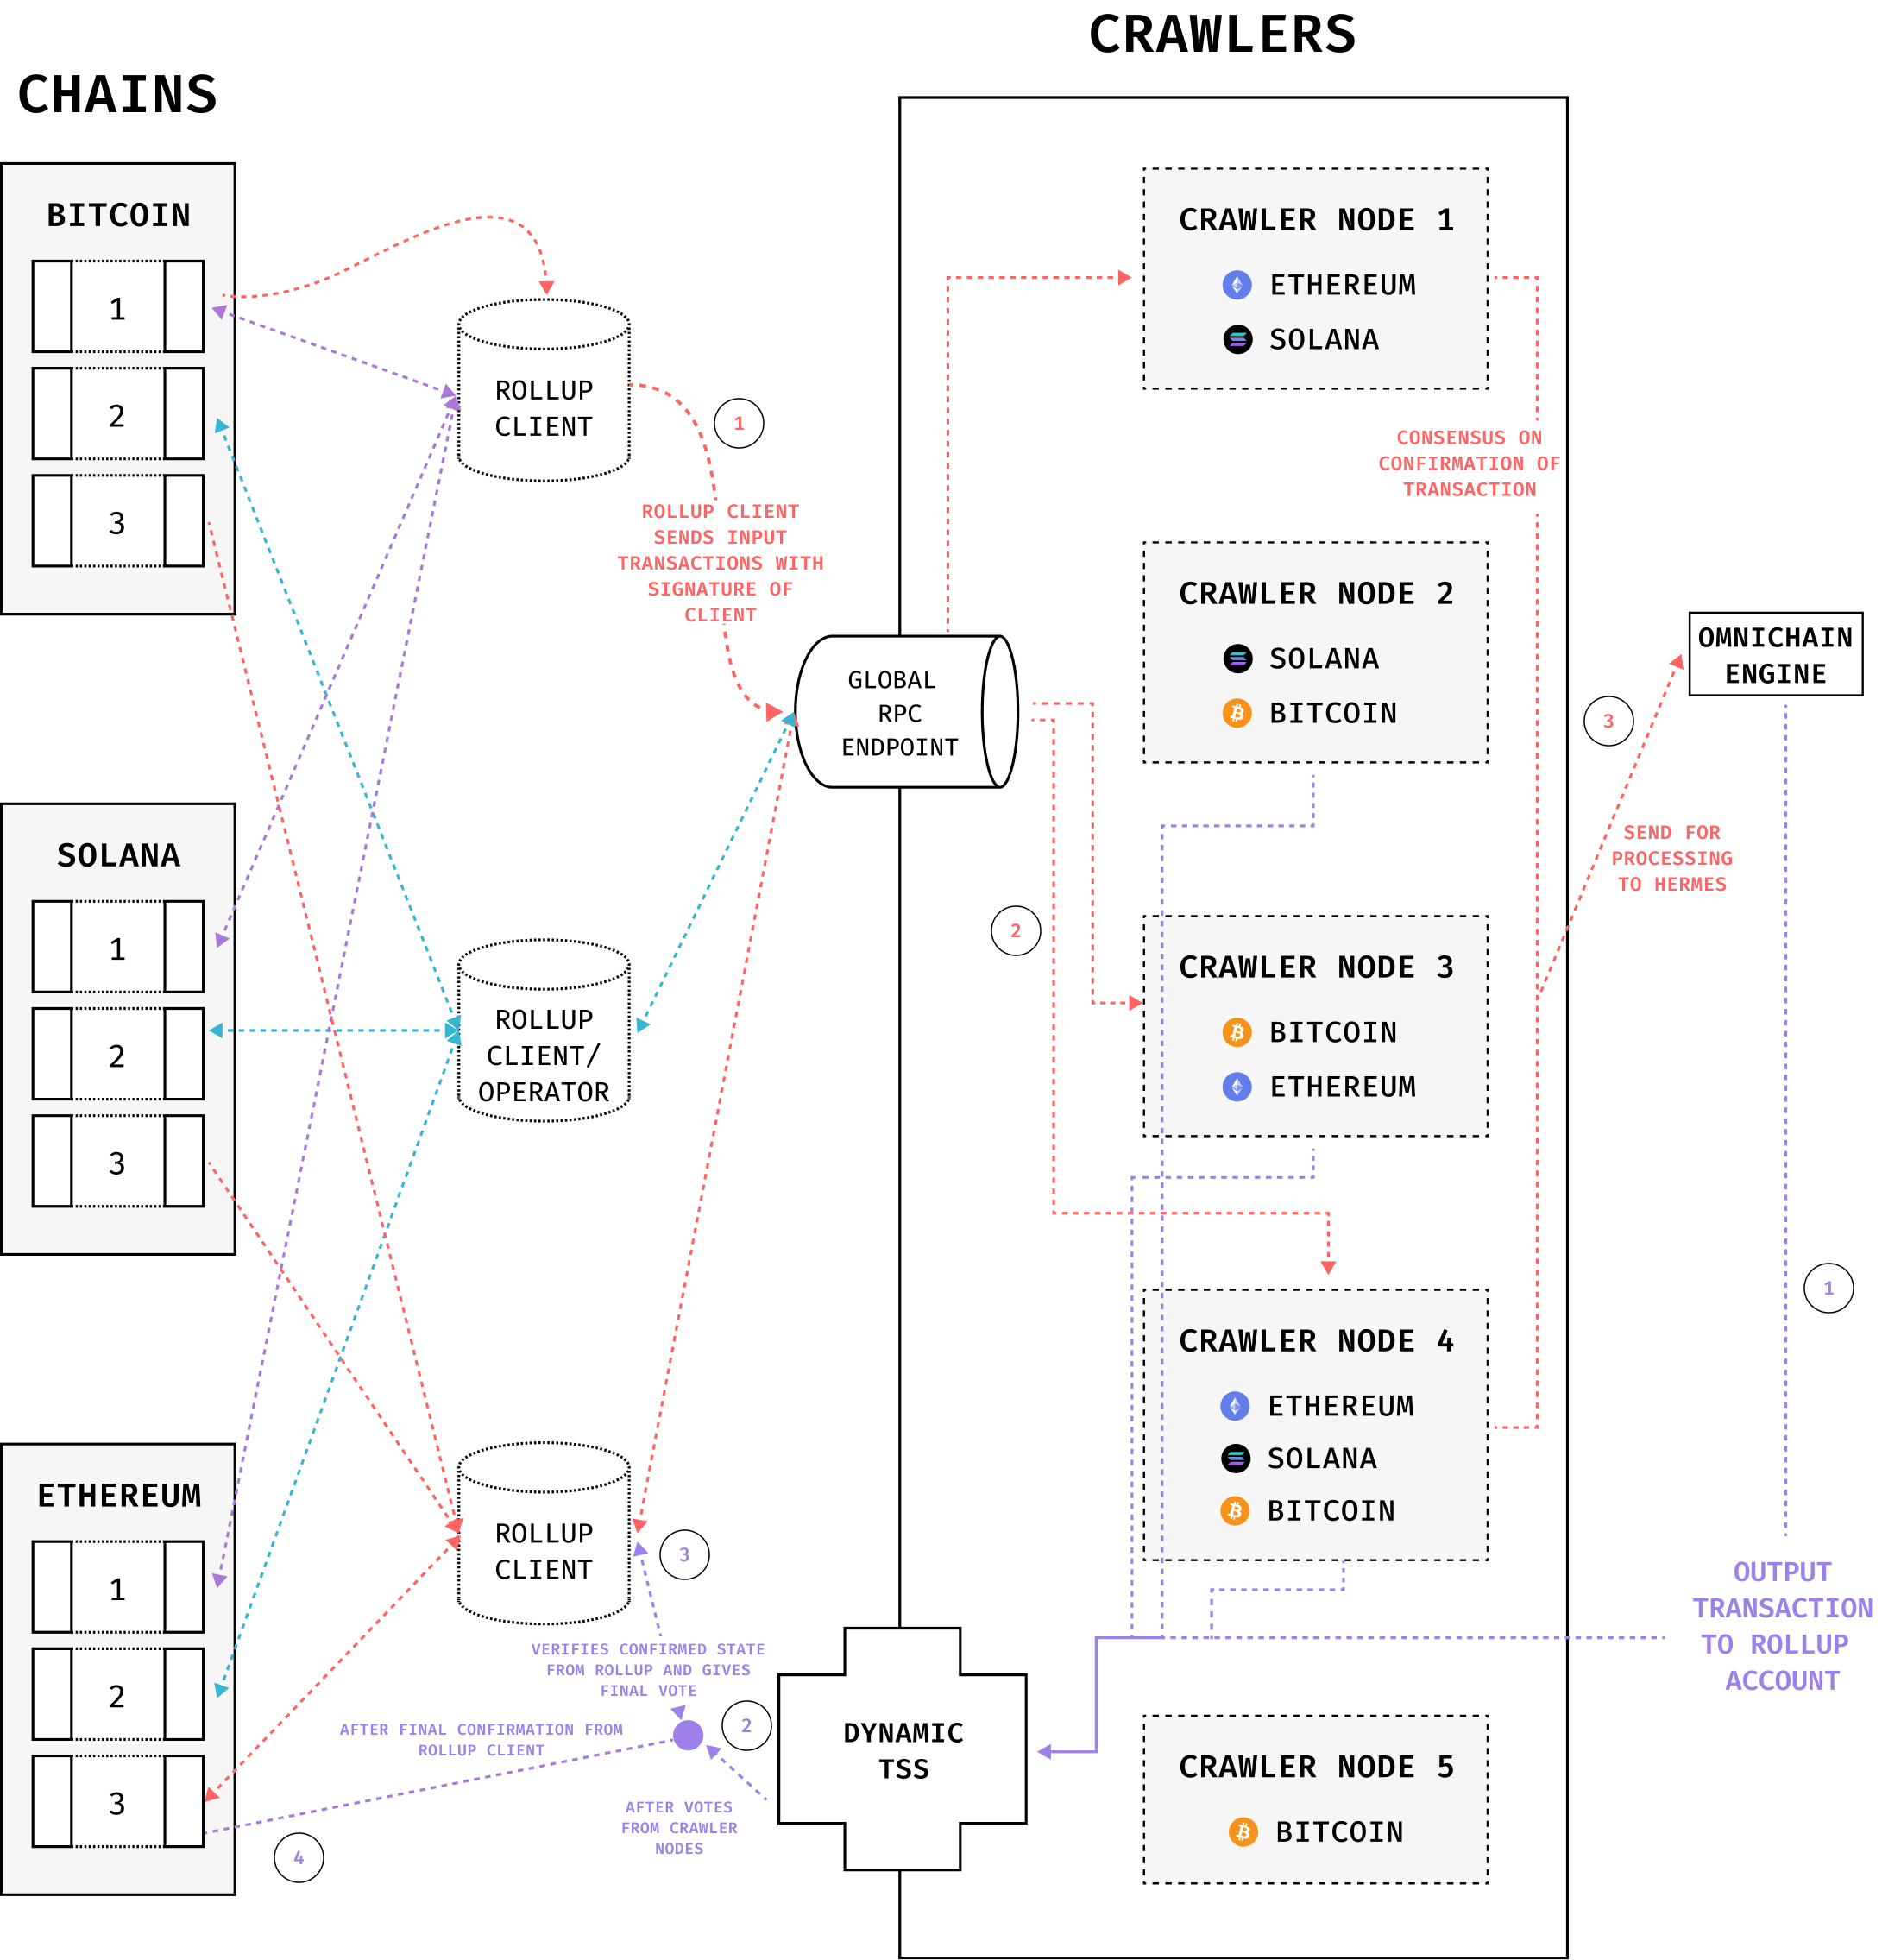
\includegraphics[width=0.99\linewidth]{figure/ragno.png}
    \caption{Ragno Network Overview}
    \label{fig:ragno}
\end{figure}

The Hermes microservice publishes these filtered transactions as preconfirmations on the Hermes chain, which acts as a checkpoint to ensure that the transactions have been identified and validated for further processing. Block creation is governed by the Tendermint consensus protocol, which requires consensus among crawlers. An incoming transaction is recorded only when a majority of Crawlers receive identical transaction data from different operators.  

Before settlement, the protocol confirms that the corresponding transaction on the source chain has been successfully executed. This verification is achieved by cross-referencing the transaction’s status on the source chain, either using a proof generated by the Prover Network or through a direct query via Hermes.

The Narada microservice monitors outbound transactions destined for the target chain. These transactions are signed using the GG20 threshold ECDSA Signature Scheme (TSS), ensuring cryptographic security and resilience against single points of failure. After signing, the transactions are verified by the crawler to ensure integrity. Once validated, they are forwarded to the target chain for settlement. The target chain executes the transaction and updates its state based on the provided payload.

Upon successful execution on the target chain, the Hermes chain records the transaction's final state. This record is updated to reflect the successful completion of cross-chain communication and settlement, thus completing the transaction lifecycle.

\subsubsection{Operator Registration}

The registration process for operators in the Ragno network ensures a secure and decentralized mechanism to accept participants who play a critical role in maintaining cross-chain communication. The first step involves staking \$DOJ tokens, a requirement that aligns operator incentives with the goals of the network. Operators use the `\textsf{createOperator}` functionality to stake the tokens, which not only secures their participation but also adds them to the set of operators maintained on the Hermes chain. This stake mechanism guarantees commitment and mitigates malicious behavior within the ecosystem.  

Once onboarded, operators are required to host blockchain nodes of their chosen networks. These nodes facilitate the relay and validation of transactions across chains. Operators manage and register their nodes via the Operator Dashboard, which serves as a centralized interface for updating and maintaining their infrastructure. Any changes or additions to the nodes are automatically recorded in the Hermes chain through the dashboard, ensuring transparency and up-to-date records.  

To maintain synchronization and efficiency, crawler nodes continuously monitor the Hermes chain for operator-related events, such as updates to the operator set or node configurations. These events are filtered and stored locally by crawlers, enabling rapid querying and reducing overhead during data synchronization. This robust monitoring mechanism ensures that the Ragno network is up-to-date with the latest operator and node information, providing a reliable backbone for cross-chain communication.

\subsubsection{Data Fetching Process}
The data fetching process in the Ragno Network employs a structured, secure, and pull-based mechanism to ensure efficient and authenticated communication between crawler nodes and operator nodes. This process is based on the Hermes chain, which plays a central role in managing mappings, ensuring fairness, and maintaining the integrity of the data flow.

\textbf{Pull-Based Mechanism and Pairing List (PL)}

The crawler nodes operate on a pull-based system, periodically querying the operator nodes to retrieve the latest blockchain data. To coordinate these interactions, the Hermes Chain publishes a Pairing List (PL) every 200 blocks. The PL assigns specific crawler nodes to designated operator nodes, defining which crawlers are responsible for fetching data from which operators. This mapping ensures an equitable distribution of workload across the network and prevents unnecessary redundancies.

The PL is aggregated based on submissions from crawlers, finalized on the Hermes Chain, and then disseminated to all crawler nodes. Crawlers use this final PL to determine their assigned operator and initiate data requests. Crawlers can only fetch data from operators they are mapped to, ensuring strict adherence to PL guidelines and preventing unauthorized data access.

\textbf{Authenticated Requests from Crawlers to Operators}

Once the PL assigns mappings, crawler nodes send authenticated data requests to their designated operators. These requests include the following components:  

- Request Metadata: Contains the specific block range or transaction data that are being queried.  

- Signature: The request is digitally signed by the crawler using its private key.  

- Public Key Reference: Includes the crawler’s public key for verification.  

Operators verify the authenticity of the requests using the public key provided in the request, mapping it against the authorized pairing list published on the Hermes chain. This ensures that only legitimate crawlers, as defined by the PL, can request data from an operator. Signature verification is performed using cryptographic methods to confirm that the request has not been tampered with and originates from the intended crawler.

\textbf{Role of the Operator Gateway Server}

Each operator node is equipped with a gateway server that acts as a secure intermediary for data exchange between the operator’s blockchain nodes and the crawler nodes. The gateway server provides several critical functionalities:  
\begin{itemize}
    \item Authentication: Verifies incoming crawler requests by cross-checking the public key in the request with the PL.  

    \item Signature Verification: Ensures the integrity of the request by validating the digital signature against the crawler’s public key.  

    \item Rate Limiting and Caching: Implements mechanisms to prevent overloading and ensures fair access to data by all assigned crawlers.  

    \item Data Delivery: Responds to validated requests by providing the required blockchain data, such as blocks or transactions.
\end{itemize}

\textbf{Data Flow and Processing}

Once authenticated, the crawler retrieves the block and transaction data from the operator node. The data fetched by the crawler are processed locally to filter transactions relevant to Dojima cross-chain interactions. The transactions pertaining to private rollup or applications will be fetched by a dedicated client who will pass it on to crawler for further processing. These filtered transactions are then sent to the Hermes chain for further validation and processing. This systematic approach ensures that only verified relevant cross-chain transactions are propagated through the network, maintaining data integrity and operational efficiency. Operators earn rewards for their contributions, with rewards calculated based on the compute resources and data they provide, incentivizing active participation and reliability.

By combining a structured pairing mechanism, authenticated communication, and robust data handling, the Ragno network ensures a seamless and secure flow of cross-chain data.

\subsubsection{Outbound Transactions}
When a block is created in the Hermes chain, outbound transactions are generated for those that require cross-chain actions. Each outbound transaction is accompanied by a validity proof to verify its correctness and, when necessary, a source chain execution proof to confirm the transaction’s successful processing on the originating chain. These safeguards ensure the integrity and reliability of cross-chain operations.
Signing Mechanism for Outbound Transactions

Outbound transactions are categorized according to their destination:

\begin{itemize}
    \item \textsf{L1 Chain Settlement Transactions:}
    
    For transactions that settle on Layer 1 (L1) chains, the Narada microservice employs the threshold ECDSA protocol to generate secure digital signatures. Initially, for each vault associated with an L1 chain, the validators collaboratively run a (k, n)-threshold ECDSA key generation algorithm. This process produces a shared public key for the vault and distributes the corresponding private key shares among the validators securely. For private vaults, the client starts the dynamic TSS key generation process and distributes some key shares to the validators.
        
    When an L1 settlement transaction requires signature, the validators collaboratively, along with the client whenever required, perform the threshold signing process. If the transaction gathers signatures from at least the threshold number (k) of validators, the client's signature is necessary in case of private vault, it is finalized and forwarded to the respective L1 chain for execution.

    \item \textsf{Other Transaction Types:}

    For non-L1 settlement transactions, such as roll-up-related operations, Narada initiates a consensus protocol instead of threshold signing. The validaters collectively verify and approve the transaction, generating a consensus certificate to attest to its validity. The transaction, along with the consensus certificate, is forwarded to the corresponding roll-up or settlement layer for execution.
\end{itemize}

\textbf{Post-Execution Validation and Recording}

Once an outbound transaction is executed on its respective chain, crawlers seek the transaction’s execution status through operator nodes. Operators continuously monitor the target chain and relay execution data to crawler nodes assigned by the Pairing List (PL). The execution details are recorded on the Hermes chain as a final confirmation of the transaction’s cross-chain execution. This ensures the transaction's lifecycle is tracked comprehensively, providing transparency and traceability for all stakeholders.